\documentclass[12pt, a4paper]{article}
\usepackage{epsfig}
\usepackage{subfigure}
%\usepackage{amscd}
\usepackage{amssymb}
\usepackage{amsbsy}
\usepackage{amsthm}
%\usepackage[dvips]{graphicx}
\usepackage{framed}
\usepackage{amsmath}

\usepackage{graphicx}

\usepackage{natbib}
\bibliographystyle{chicago}
%\usepackage{vmargin}
%\usepackage{index}
% left top textwidth textheight headheight
% headsep footheight footskip
%\setmargins{3.0cm}{2.5cm}{15.5 cm}{22cm}{0.5cm}{0cm}{1cm}{1cm}
\renewcommand{\baselinestretch}{1.5}
\pagenumbering{arabic}
\theoremstyle{plain}
\newtheorem{theorem}{Theorem}[section]
\newtheorem{corollary}[theorem]{Corollary}
\newtheorem{ill}[theorem]{Example}
\newtheorem{lemma}[theorem]{Lemma}
\newtheorem{proposition}[theorem]{Proposition}
\newtheorem{conjecture}[theorem]{Conjecture}
\newtheorem{axiom}{Axiom}
\theoremstyle{definition}
\newtheorem{definition}{Definition}[section]
\newtheorem{notation}{Notation}
\theoremstyle{remark}
\newtheorem{remark}{Remark}[section]
\newtheorem{example}{Example}[section]
\renewcommand{\thenotation}{}
\renewcommand{\thetable}{\thesection.\arabic{table}}
\renewcommand{\thefigure}{\thesection.\arabic{figure}}

%opening
\title{Residual Analysis for Linear and LME Models with \texttt{R}}
\author{Dublin \texttt{R}}





\begin{document}

\maketitle

\tableofcontents

Below the table on the left shows inputs and outputs from a simple linear regression analysis, and the chart on the right displays the residual (e) and independent variable (X) as a residual plot.

%x	60	70	80	85	95
%y	70	65	70	95	85
%ŷ	65.411	71.849	78.288	81.507	87.945
%e	4.589	-6.849	-8.288	13.493	-2.945
% Image of residual plot
\newpage
The residual plot shows a fairly random pattern - the first residual is positive, the next two are negative, the fourth is positive, and the last residual is negative. This random pattern indicates that a linear model provides a decent fit to the data.

Below, the residual plots show three typical patterns. The first plot shows a random pattern, indicating a good fit for a linear model. The other plot patterns are non-random (U-shaped and inverted U), suggesting a better fit for a non-linear model.

		
%Random pattern	Non-random: U-shaped	Non-random: Inverted U
In the next lesson, we will work on a problem, where the residual plot shows a non-random pattern. And we will show how to "transform" the data to use a linear model with nonlinear data.

%----------------------------------------------------------------------------------------------%
\newpage
%http://blog.minitab.com/blog/adventures-in-statistics/why-you-need-to-check-your-residual-plots-for-regression-analysis
In the graph above, you can predict non-zero values for the residuals based on the fitted value. For example, a fitted value of 8 has an expected residual that is negative. Conversely, a fitted value of 5 or 11 has an expected residual that is positive.

The non-random pattern in the residuals indicates that the deterministic portion (predictor variables) of the model is not capturing some explanatory information that is “leaking” into the residuals. The graph could represent several ways in which the model is not explaining all that is possible. 

Possibilities include:

\begin{itemize}
\item A missing variable
\item A missing higher-order term of a variable in the model to explain the curvature
\item A missing interction between terms already in the model
\end{itemize}


Identifying and fixing the problem so that the predictors now explain the information that they missed before should produce a good-looking set of residuals!

In addition to the above, here are two more specific ways that predictive information can sneak into the residuals:

The residuals should not be correlated with another variable. If you can predict the residuals with another variable, that variable should be included in the model. In Minitab’s regression, you can plot the residuals by other variables to look for this problem.


\subsubsection{Autocorrelation} 
Adjacent residuals should not be correlated with each other (\textbf{autocorrelation}). If you can use one residual to predict the next residual, there is some predictive information present that is not captured by the predictors. Typically, this situation involves time-ordered observations. 

For example, if a residual is more likely to be followed by another residual that has the same sign, adjacent residuals are positively correlated. You can include a variable that captures the relevant time-related information, or use a time series analysis. 

\subsubsection{Durbin-Watson Test for Autocorrelated Errors}
The \textbf{\textit{Durbin-Watson} }procedure is commonly used to to test for autocorrelationof residuals.

\begin{framed}
\begin{verbatim}
attach(mtcars)
 FitMod <- lm(mpg~wt+cyl)

# library(car)
durbinWatsonTest(FitMod)

\end{verbatim}
\end{framed}
\begin{verbatim}
> durbinWatsonTest(FitMod)
 lag Autocorrelation D-W Statistic p-value
   1       0.1302185      1.671096   0.252
 Alternative hypothesis: rho != 0
\end{verbatim}
\newpage

% http://polisci.msu.edu/jacoby/icpsr/regress3/lectures/week3/11.Outliers.pdf
%---------------------------------------------------------------------------------------------%
\newpage
\section{Standardization and Studentization}
\subsection{Standardization} %1.4.1

A random variable is said to be standardized if the difference from its mean is scaled by its standard deviation. The residuals above have mean zero but their variance is unknown, it depends on the true values of $\theta$. Standardization is thus not possible in practice.

\subsection{Studentization} %1.4.2
Instead, you can compute studentized residuals by dividing a residual by an estimate of its standard deviation. 

\subsection{Internal and External Studentization} %1.4.3
If that estimate is independent of the $i-$th observation, the process is termed \emph{external studentization}`external studentization'. This is usually accomplished by excluding the $i-$th observation when computing the estimate of its standard error. If the observation contributes to the
standard error computation, the residual is said to be \emph{internally studentization}internally studentized.

Externally \emph{studentized residual} studentized residual require iterative influence analysis or a profiled residuals variance.

\subsection{Computation}%1.4.4

%The computation of internally studentized residuals relies on the diagonal entries of $\boldsymbol{V} (\hat{\theta})$ - $\boldsymbol{Q} (\hat{\theta})$, where $\boldsymbol{Q} (\hat{\theta})$ is computed as

\[ \boldsymbol{Q} (\hat{\theta}) = \boldsymbol{X} ( \boldsymbol{X}^{\prime}\boldsymbol{Q} (\hat{\theta})^{-1}\boldsymbol{X})\boldsymbol{X}^{-1} \]

\subsection{Pearson Residual}%1.4.5

Another possible scaled residual is the \index{Pearson residual} `Pearson residual', whereby a residual is divided by the standard deviation of the dependent variable. The Pearson residual can be used when the variability of $\hat{\beta}$ is disregarded in the underlying assumptions.






\newpage
\section{Regression Diagnostics with \texttt{R} }
% http://www.statmethods.net/stats/rdiagnostics.html

An excellent review of regression diagnostics is provided in John Fox's aptly named \textit{Overview of Regression Diagnostics}. Dr. Fox's car package provides advanced utilities for regression modeling.

\begin{verbatim}
(1) Fox, John. (1991). Regression Diagnostics: An Introduction. Sage Publications.
\end{verbatim}

\begin{framed}
\begin{verbatim}
# Assume that we are fitting a multiple linear regression
# on the MTCARS data
library(car)
fit <- lm(mpg~disp+hp+wt+drat, data=mtcars)

\end{verbatim}
\end{framed}


\subsection{Outliers}

Assessment of Outliers can be carried out using the \texttt{outlierTest} function.

\begin{framed}
\begin{verbatim}
outlierTest(fit) # Bonferonni p-value for most extreme obs
qqPlot(fit, main="QQ Plot") #qq plot for studentized resid 
leveragePlots(fit) # leverage plots
\end{verbatim}
\end{framed}
\subsection{Added Variable Plots}
\begin{framed}
\begin{verbatim}
# added variable plots 
av.Plots(fit)
\end{verbatim}
\end{framed}

\subsection{Non-constant Error Variance}
\begin{framed}
\begin{verbatim}

# Evaluate homoscedasticity
# non-constant error variance test
ncvTest(FitMod)
# plot studentized residuals vs. fitted values 
spreadLevelPlot(FitMod)
\end{verbatim}
\end{framed}

\begin{verbatim}
> ncvTest(FitMod)
Non-constant Variance Score Test 
Variance formula: ~ fitted.values 
Chisquare = 3.330027    Df = 1     p = 0.06802577 
\end{verbatim}

%mtcarsSpreadLevel Plot here

\begin{figure}[h!]
\centering
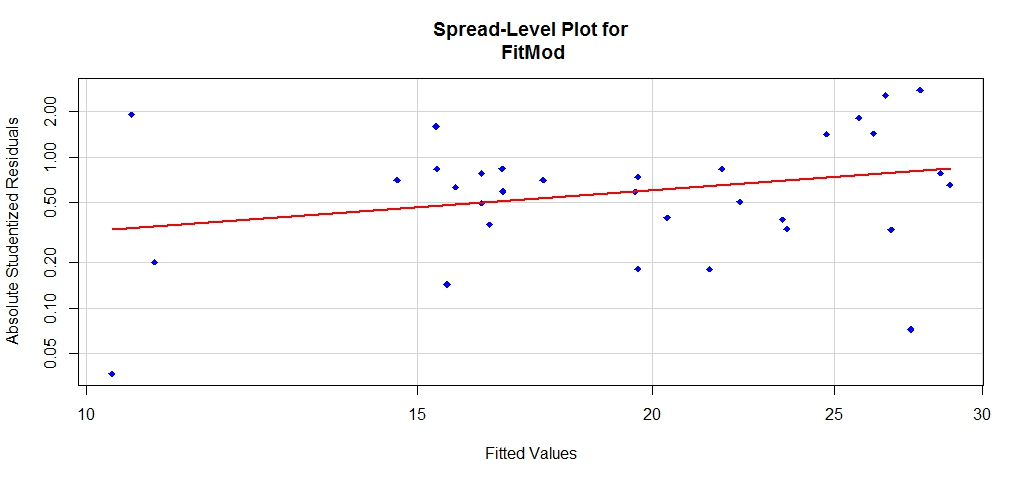
\includegraphics[width=0.7\linewidth]{./mtcarsSpreadLevelPlot}
\label{mtcarsSpreadLevelPlot}
\end{figure}


\begin{verbatim}
Suggested power transformation:  0.08866484 
\end{verbatim}

\subsection{Influential Observations}
\begin{framed}
\begin{verbatim}
# Influential Observations

# Cook's D plot
# identify D values > 4/(n-k-1) 
cutoff <- 4/((nrow(mtcars)-length(fit$coefficients)-2)) 
plot(fit, which=4, cook.levels=cutoff)
# Influence Plot 
influencePlot(fit,	 id.method="identify", main="Influence Plot", sub="Circle size is proportial to Cook's Distance" )
\end{verbatim}
\end{framed}
%-------------------------------------------------------------- %

\section{Case Deletion} %1.14
Case-deleted analysis is a popular method for evaluating the influence of a subset of cases on inference.

\textbf{Cite: CPJ} develops case-deletion diagnostics for detecting influential observations in mixed linear models. Diagnostics for both fixed effects and variance components are proposed. Computational formulas are given that make the procedures feasible. The methods are illustrated using examples. 

\subsection{Case Deletion Diagnostic Statistics}
% http://support.sas.com/documentation/cdl/en/statug/63033/HTML/default/viewer.htm#statug_genmod_sect045.htm

For ordinary generalized linear models, regression diagnostic statistics developed by Williams (1987) are commonly used in statistical platforms such as SS. These diagnostics measure the influence of an individual observation on model fit, and generalize the one-step diagnostics developed by Pregibon (1981) for the logistic regression model for binary data.
Preisser and Qaqish (1996) further generalize regression diagnostics to apply to models for correlated data fit by generalized estimating equations (GEEs), where the influence of entire clusters of correlated observations is measured.


\subsection{Matrix Notation for  Case deletion notation} %1.14.1

For notational simplicity, $\boldsymbol{A}(i)$ denotes an $n \times m$ matrix $\boldsymbol{A}$ with the $i$-th row
removed, $a_i$ denotes the $i$-th row of $\boldsymbol{A}$, and $a_{ij}$ denotes the $(i, j)-$th element of $\boldsymbol{A}$.

\subsection{Partitioning Matrices} %1.14.2
Without loss of generality, matrices can be partitioned as if the $i-$th omitted observation is the first row; i.e. $i=1$.

%---------------------------------------------------------------------------%
\newpage
\subsection{CPJ's Three Propositions} %1.15
%-----------------------------%


\subsubsection{Proposition 1}

\[
\boldsymbol{V}^{-1} =
\left[ \begin{array}{cc}
\nu^{ii} & \lambda_{i}^{\prime}  \\
\lambda_{i} & \Lambda_{[i]}
\end{array}\right] \]


\[\boldsymbol{V}_{[i]}^{-1} = \boldsymbol{\Lambda}_{[i]} - { \lambda_{i} \lambda_{i} ^{\prime} \over \lambda_{i} } \]

%-----------------------------%
\subsection{Proposition 2}

\begin{itemize}
\item[(i)] $ \boldsymbol{X}_{[i]}^{T}\boldsymbol{V}^{-1}_{[i]}\boldsymbol{X}_{[i]}$ = $\boldsymbol{X}^{\prime}\boldsymbol{V}^{-1}\boldsymbol{X}$
\item[(ii)] = $(\boldsymbol{X}^{\prime}\boldsymbol{V}^{-1}\boldsymbol{Y})^{-1}$
\item[(iii)] $ \boldsymbol{X}_{[i]}^{T}\boldsymbol{V}^{-1}_{[i]}\boldsymbol{Y}_{[i]}$ = $\boldsymbol{X}^{\prime}\boldsymbol{V}^{-1}\boldsymbol{Y}$
\end{itemize}
%-----------------------------%
\subsection{Proposition 3}
This proposition is similar to the formula for the one-step Newtown Raphson estimate of the logistic regression coefficients given by Pregibon (1981) and discussed in Cook Weisberg.
\newpage
\newpage
\section{Robust Regression (Optional Section)}

Robust regression is an alternative to ordinary least squares regression (OLS , the type of regression we have studied thus far) when data is contaminated with outliers or influential observations and it can also be used for the purpose of detecting influential observations.


\begin{framed}
\begin{verbatim}
FitAll = lm(Taste ~ Acetic + H2S + Lactic)
plot(FitAll)
\end{verbatim}
\end{framed}
This will produce a set of four plots: residuals versus fitted values, a Q-Q plot of standardized residuals, a scale-location plot (square roots of standardized residuals versus fitted values, and a plot of residuals versus leverage that adds bands corresponding to Cook's distances of 0.5 and 1. 

Using the plot to get a detailed interpretation of how well the model fits is beyond the scope of this module. However it is worth noting that plots identify particular observations that may warrant re-examination. 

\textbf{Remarks :} 
% OLD MA4605 Notes
The plots actually indicate the fitted model is actually quite good. The trend lines in the first and third plots demonstrate constant variance, and in the case of the first, the trend line through the centre of the plot  follows the X=0 line quite well.

The Q-Q plot (i.e. the second plot) indicates that the assumption of normality is vindicated.
The last plot indicates the no observations have unusually high Cook’s Distances values.  No observations are beyond the 0.5 (red line) threshold.

Robust regression is an alternative to least squares regression when data are contaminated with outliers or influential observations, and it can also be used for the purpose of detecting influential observation

% IMAGES HERE

Additionally I have added a line plot of the Cook’s Distance values. Which observations have the highest values for Cook’s Distance?

\begin{framed}
\begin{verbatim}
plot(cooks.distance(FitAll),type="b",pch=18,col="red")
\end{verbatim}
\end{framed}





%------------------------------------------------------------------------------------%
\subsection{The stackloss data set}
%Used in "rlm" help file
Brownlee's Stack Loss Plant Data contains operational data of a plant for the oxidation of ammonia to nitric acid.

The variables are: 
\begin{itemize}
\item	Air Flow	 Flow of cooling air
\item	Water Temp	 Cooling Water Inlet Temperature
\item	Acid Conc.	 Concentration of acid [per 1000, minus 500]
\item	stack.loss	 Stack loss
\end{itemize}

\subsection{Fitting a robust model (\texttt{rlm}}
%-------------------------------------%
\begin{framed}
\begin{verbatim}
summary(rlm(stack.loss ~ ., data = stackloss))
\end{verbatim}
\end{framed}
%-------------------------------------%
\begin{verbatim}
> summary(rlm(stack.loss ~ ., stackloss))

Call: rlm(formula = stack.loss ~ ., data = stackloss)
Residuals:
     Min       1Q   Median       3Q      Max 
-8.91753 -1.73127  0.06187  1.54306  6.50163 

Coefficients:
            Value    Std. Error t value 
(Intercept) -41.0265   9.8073    -4.1832
Air.Flow      0.8294   0.1112     7.4597
Water.Temp    0.9261   0.3034     3.0524
Acid.Conc.   -0.1278   0.1289    -0.9922

Residual standard error: 2.441 on 17 degrees of freedom
\end{verbatim}
%-------------------------------------%
\begin{framed}
\begin{verbatim}
 rlm(stack.loss ~ ., stackloss, psi = psi.hampel, init = "lts")
\end{verbatim}
\end{framed}
%-------------------------------------%
\begin{verbatim}
> rlm(stack.loss ~ ., stackloss, psi = psi.hampel, init = "lts")
Call:
rlm(formula = stack.loss ~ ., data = stackloss, psi = psi.hampel, 
    init = "lts")
Converged in 10 iterations

Coefficients:
(Intercept)    Air.Flow  Water.Temp  Acid.Conc. 
-40.4748037   0.7410863   1.2250703  -0.1455242 

Degrees of freedom: 21 total; 17 residual
Scale estimate: 3.09 
\end{verbatim}
%-------------------------------------%
\subsection{Using Other \textit{Psi} Operators}

Fitting is done by \textbf{\emph{iterated re-weighted least squares (IWLS).}}

Psi functions are supplied for the Huber, Hampel and Tukey bisquare proposals as psi.huber, \texttt{psi.hampel} and \textbf{psi.bisquare}. Huber's corresponds to a convex optimization problem and gives a unique solution (up to collinearity). The other two will have multiple local minima, and a good starting point is desirable.



\begin{itemize}
\item huber
\item bisquare
\item hampel

\end{itemize}

\begin{framed}
\begin{verbatim}
 rlm(stack.loss ~ ., stackloss, psi = psi.bisquare)
\end{verbatim}
\end{framed}
\begin{verbatim}
Call:
rlm(formula = stack.loss ~ ., data = stackloss, psi = psi.bisquare)
Converged in 11 iterations

Coefficients:
(Intercept)    Air.Flow  Water.Temp  Acid.Conc. 
-42.2852537   0.9275471   0.6507322  -0.1123310 

Degrees of freedom: 21 total; 17 residual
Scale estimate: 2.28 
\end{verbatim}


\subsection{Implementation of Robust Regression}
\begin{itemize}
\item When fitting a least squares regression, we might find some outliers or high leverage data points.  We have decided that these data points are not data entry errors, neither they are from a different population than most of our data. So we have no proper reason to exclude them from the analysis.  

\item Robust regression might be a good strategy since it is a compromise between excluding these points entirely from the analysis and including all the data points and treating all them equally in OLS regression. The idea of robust regression is to weigh the observations differently based on how well behaved these observations are.

\item 
The idea of robust regression is to weigh the observations differently based on how well behaved these observations are. Roughly speaking, it is a form of weighted and reweighted least squares regression (i.e. a two step process , first fitting a linear model, then a robust model to correct for the influence of outliers).
\item 
Robust regression is done by iterated re-weighted least squares (IRLS). The rlm command in the MASS package command implements several versions of robust regression.
\item 
There are several weighting functions that can be used for IRLS. We are going to first use the Huber weights in this example. We will then look at the final weights created by the IRLS process. This can be very useful. 
\item 
Also we will look at an alternative weighting approach to Huber’s weighting – called \textbf{Bisquare weighting}. 
\end{itemize}
%-----------------------------------------%
\subsubsection{Huber Weighting}
In Huber weighting, observations with small residuals get a weight of 1 and the larger the residual, the smaller the weight. This is defined by the weight function


\begin{eqnarray}
w(e) = 1 for |e| \leq k  \\
w(e) = \frac{k}{|e|} for |e| > k
\end{eqnarray}


The value $k$ for the Huber method is called a \textbf{\textit{tuning constant}}; smaller values of k produce more resistance to outliers, but at the expense of lower efficiency when the errors are normally distributed.

The tuning constant is generally picked to give reasonably high efficiency in the normal case; in particular,$ k = 1.345\sigma$ for the Huber’s method, where $\sigma$ is the standard deviation of the errors) produce 95-percent efficiency when the errors are normal, and still offer protection against outliers.

%(Bisquare Weighting is very similar).

\begin{framed}
\begin{verbatim}
library(MASS)
FitAll.rr = rlm(Taste ~ Acetic + H2S + Lactic)
\end{verbatim}
\end{framed}

\begin{verbatim}
> summary(FitAll.rr)

Call: rlm(formula = Taste ~ Acetic + H2S + Lactic)
Residuals:
    Min      1Q  Median      3Q     Max 
-16.163  -5.612  -1.153   5.487  27.106 

Coefficients:
            Value    Std. Error t value 
(Intercept) -20.7529  20.1001    -1.0325
Acetic       -1.5331   4.5422    -0.3375
H2S           4.0515   1.2715     3.1864
Lactic       20.1459   8.7885     2.2923

Residual standard error: 8.471 on 26 degrees of freedom
\end{verbatim}

Regression Equation: 
\[ \hat{Taste} = -20.75 -1.53 Acetic + 4.05 H2S + 20.14 Lactic\]
From before, we noticed that observations 15 , 12 and 8 were influential in the determination of the coefficients. The following table indicates the weight given to each observation when using robust regression.  

We can see that roughly, as the absolute residual goes down, the weight goes up. In other words, cases with a large residuals tend to be down-weighted.

%(You do not need to know how to implement the code used to generate this table, but we will be looking at how to construct data frames later in the course.)

\begin{framed}
\begin{verbatim}
> hweights <- data.frame(Taste = Taste, resid = FitAll.rr$resid,
+     weight = FitAll.rr$w)
> hweights2 <- hweights[order(FitAll.rr$w), ]
>
\end{verbatim}
\end{framed}

\begin{verbatim}
> hweights2[1:15, ]
   Taste      resid    weight
15  54.9  27.105636 0.4203556
12  57.2  17.518919 0.6504044
8   21.9 -16.162753 0.7049043
3   39.0  14.318512 0.7957592
18   6.4 -13.609277 0.8371707
28   0.7 -11.410452 0.9985018
1   12.3   9.990965 1.0000000
2   20.9  -1.692664 1.0000000
4   47.9  10.648009 1.0000000
5    5.6  -1.866642 1.0000000
6   25.9   2.632602 1.0000000
7   37.3   5.744433 1.0000000
9   18.1   4.775657 1.0000000
10  21.0   1.048052 1.0000000
11  34.9   5.723592 1.0000000
\end{verbatim}
\subsubsection{Implementation with Bisquare Weighting}
Implementing with bisquare weighting simply requires the specification of the additional argument, as per the code below, highlighted in green)
\begin{framed}
\begin{verbatim}
> FitAll.rr.2 = rlm(Taste ~ Acetic + H2S + Lactic, psi = psi.bisquare)
\end{verbatim}
\end{framed}
\begin{verbatim}
> summary(FitAll.rr.2)

Call: rlm(formula = Taste ~ Acetic + H2S + Lactic, psi = psi.bisquare)
Residuals:
     Min       1Q   Median       3Q      Max 
-15.7034  -5.1552  -0.9793   5.6933  27.7661 

Coefficients:
            Value    Std. Error t value 
(Intercept) -17.7730  20.7031    -0.8585
Acetic       -2.2650   4.6784    -0.4841
H2S           4.0569   1.3096     3.0977
Lactic       20.6885   9.0522     2.2855

Residual standard error: 7.878 on 26 degrees of freedom
\end{verbatim}
%Regression Equation :

%Taste* = -17.77 -2.26 Acetic + 4.05 H2S + 20.68 Lactic


Weights using Bisquare estimator.

\begin{verbatim}
> hweights2[1:15, ]
   Taste      resid    weight
15  54.9  27.766087 0.1884633
12  57.2  18.182810 0.5735669
8   21.9 -15.703388 0.6707319
3   39.0  14.384429 0.7193235
18   6.4 -13.462286 0.7516310
28   0.7 -11.190438 0.8246092
19  18.0 -11.112316 0.8269297
4   47.9  10.860173 0.8343637
1   12.3   9.852297 0.8625704
20  38.9  -8.952091 0.8858015
14  25.9   8.588121 0.8946576
30   5.5  -8.019522 0.9078077
7   37.3   6.329446 0.9420556
11  34.9   5.999726 0.9478611
13   0.7  -5.470990 0.9565447
\end{verbatim}

\subsubsection{Conclusion}
We can see that the weight given to some observations is dramatically lower using the bisquare weighting function than the Huber weighting function and the coefficient estimates from these two different weighting methods differ. 
When comparing the results of a regular OLS regression and a robust regression, if the results are very different, you will most likely want to use the results from the robust regression. 
Large differences suggest that the model parameters are being highly influenced by outliers. Different functions have advantages and drawbacks. Huber weights can have difficulties with severe outliers, and bisquare weights can have difficulties converging or may yield multiple solutions. 




%-------------------------------------------------------------- %
\newpage
\section{Residual Analysis for GLMs (Optional Section)}





\subsection{Pearson and Deviance Residuals} 
% https://v8doc.sas.com/sashtml/insight/chap39/sect55.htm

Pearson Residuals





The Pearson residual is the raw residual divided by the square root of the variance function $V(\mu).$
The Pearson residual is the individual contribution to the Pearson $\chi^2$ statistic. 

For a binomial distribution with mi trials in the ith observation, it is defined as

\[ r_{Pi} = \sqrt{ m_{i}}
 \frac{r_{i}}{\sqrt{V(\hat{ \mu_{i}})}} \]
For other distributions, the Pearson residual is defined as

\[ r_{Pi} = \frac{r_{i}}{\sqrt{V(\hat{ \mu_{i}})}}\]
The Pearson residuals can be used to check the model fit at each observation for generalized linear models. 
%These residuals are stored in variables named RP_yname for each response variable, where yname is the response variable name. 
The standardized and studentized Pearson residuals are
\[
r_{Psi} = \frac{r_{Pi}}{\sqrt{\hat{ \phi} (1- h_{i})} } \]
\[ r_{Pti} = \frac{r_{Pi}}{\sqrt{ \hat{ \phi}_{(i)}
 (1- h_{i})} } \]



The \textbf{deviance residual} is the measure of deviance contributed from each observation and is given by
\[r_{Di} = \textrm{sign}( r_{i})
 \sqrt{ d_{i}}\]
where $d_i$ is the individual deviance contribution.
The deviance residuals can be used to check the model fit at each observation for generalized linear models. 

%These residuals are stored in variables named \textit{RD\_yname} for each response variable, where yname is the response variable name. 

The standardized and studentized deviance residuals are
\[
r_{Dsi} = \frac{r_{Di}}{\sqrt{\hat{ \phi} (1- h_{i})} }\]
\[r_{Dti} = \frac{r_{Di}}{\sqrt{ \hat{ \phi}_{(i)}
 (1- h_{i})}}\]
 
\newpage
 
\subsection{Diagnostics for Logistic Regression}

\subsection{Diagnostics for Poisson Regression}
%-------------------------------------------------------------- %
\newpage
\section{Residual Analysis for LME Models}
\subsection{Introduction}%1.1
In classical linear models model diagnostics have been become a required part of any statistical analysis, and the methods are commonly available in statistical packages and standard textbooks on applied regression. However it has been noted by several papers that model diagnostics do not often accompany LME model analyses.

\textbf{Cite:Zewotir} lists several established methods of analyzing influence in LME models. These methods include \begin{itemize}
\item Cook's distance for LME models,
\item \index{likelihood distance} likelihood distance,
\item the variance (information) ration,
\item the \index{Cook-Weisberg statistic} Cook-Weisberg statistic,
\item the \index{Andrews-Prebigon statistic} Andrews-Prebigon statistic.
\end{itemize}

%-------------------------------------------------------------------------------------------------------------------------------------%
\subsection{Zewotir Measures of Influence in LME Models}%2.2
%Zewotir page 161
\citet{Zewotir} describes a number of approaches to model diagnostics, investigating each of the following;
\begin{itemize}
\item Variance components
\item Fixed effects parameters
\item Prediction of the response variable and of random effects
\item likelihood function
\end{itemize}

\subsection{Cook's Distance applied to LMEs}
\begin{itemize}
\item For variance components $\gamma$: $CD(\gamma)_i$,
\item For fixed effect parameters $\beta$: $CD(\beta)_i$,
\item For random effect parameters $\boldsymbol{u}$: $CD(u)_i$,
\item For linear functions of $\hat{beta}$: $CD(\psi)_i$
\end{itemize}

\subsection{Iterative and non-iterative influence analysis for LMEs} %1.13

\textbf{Cite: Schabenberger} highlights some of the issue regarding implementing mixed model diagnostics.

A measure of total influence requires updates of all model parameters. However, this doesnt increase the procedures execution time by the same degree.

\subsection{Iterative Influence Analysis}

%----schabenberger page 8
For linear models, the implementation of influence analysis is straightforward.
However, for LME models, the process is more complex. Update formulas for the fixed effects are available only when the covariance parameters are assumed to be known. A measure of total influence requires updates of all model parameters. This can only be achieved in general is by omitting observations, then refitting the model.\textbf{Cite: Schabenberger} describes the choice between \index{iterative influence analysis} iterative influence analysis and \index{non-iterative influence analysis} non-iterative influence analysis.



%------------------------------------------------------------%
\begin{description}
\item[Random Effects]

A large value for $CD(u)_i$ indicates that the $i-$th observation is influential in predicting random effects.

\item[linear functions]
$CD(\psi)_i$ does not have to be calculated unless $CD(\beta)_i$ is large.


\item[Information Ratio]
\end{description}

%--------------------------------------------------------------%
\newpage
\section{Measures 2} %2.4

\subsection{Cook's Distance} %2.4.1
\begin{itemize}
\item For variance components $\gamma$
\end{itemize}

Diagnostic tool for variance components
\[ C_{\theta i} =(\hat(\theta)_{[i]} - \hat(\theta))^{T}\mbox{cov}( \hat(\theta))^{-1}(\hat(\theta)_{[i]} - \hat(\theta))\]

\subsection{Variance Ratio} %2.4.2
\begin{itemize}
\item For fixed effect parameters $\beta$.
\end{itemize}

\subsection{Cook-Weisberg statistic} %2.4.3
\begin{itemize}
\item For fixed effect parameters $\beta$.
\end{itemize}

\subsection{Andrews-Pregibon statistic} %2.4.4
\begin{itemize}
\item For fixed effect parameters $\beta$.
\end{itemize}
The Andrews-Pregibon statistic $AP_{i}$ is a measure of influence based on the volume of the confidence ellipsoid.
The larger this statistic is for observation $i$, the stronger the influence that observation will have on the model fit.


%---------------------------------------------------------------------------%




%------------------------------------------------------------%
\subsection{Likelihood Distance}


\citet{BA83}

\subsection{Diagnostics for LMEs with \texttt{R}}
influence.ME: Tools for detecting influential data in mixed effects models

influence.ME provides a collection of tools for detecting influential cases in generalized mixed effects models. It analyses models that were estimated using lme4. The basic rationale behind identifying influential data is that when iteratively single units are omitted from the data, models based on these data should not produce substantially different estimates. To standardize the assessment of how influential a (single group of) observation(s) is, several measures of influence are common practice, such as DFBETAS and Cook's Distance. In addition, we provide a measure of percentage change of the fixed point estimates and a simple procedure to detect changing levels of significance.


%------------------------------------------------------------------------------------------------%
% http://journal.r-project.org/archive/2012-2/RJournal_2012-2_Nieuwenhuis~et~al.pdf

You should have a look at the \texttt{R} package \textit{\textbf{influence.ME}}. It allows you to compute measures of influential data for mixed effects models generated by lme4.

An example model:
\begin{verbatim}
library(lme4)
model <- lmer(mpg ~ disp + (1 | cyl), mtcars)
\end{verbatim}

The function \texttt{influence} is the basis for all further steps:

\begin{verbatim}
library(influence.ME)
infl <- influence(model, obs = TRUE)
\end{verbatim}
Calculate Cook's distance:
\begin{verbatim}
cooks.distance(infl)
\end{verbatim}
Plot Cook's distance:
\begin{verbatim}
plot(infl, which = "cook")
\end{verbatim}
\newpage
%----------------------------------------------------------------------------------------%

\section{Case-Deletion Diagnostics for LMEs The CPJ Paper}%1.13

\subsection{Case-Deletion results for Variance components}
\textbf{Cite: CPJ}  examines case deletion results for estimates of the variance components, proposing the use of one-step estimates of variance components for examining case influence. The method describes focuses on REML estimation, but can easily be adapted to ML or other methods.

This paper develops their global influences for the deletion of single observations in two steps: a one-step estimate for the REML (or ML) estimate of the variance components, and an ordinary case-deletion diagnostic for a weighted regression problem ( conditional on the estimated covariance matrix) for fixed effects.

% Lesaffre's approach accords with that proposed by Christensen et al when applied in a repeated measurement context, with a large sample size.

\subsection{CPJ Notation} %1.13.1

\[ \boldsymbol{C} = \boldsymbol{H}^{-1} = \left[
\begin{array}{cc}
c_{ii} & \boldsymbol{c}_{i}^{\prime}\\
\boldsymbol{c}_{i} &  \boldsymbol{C}_{[i]}
\end{array} \right]
\]

\textbf{Cite: CPJ}  noted the following identity:

\[ \boldsymbol{H}_{[i]}^{-1}  = \boldsymbol{C}_{[i]} - {1 \over c_{ii}}\boldsymbol{c}_{[i]}\boldsymbol{c}_{[i]}^{\prime} \]


\textbf{Cite: CPJ} use the following as building blocks for case deletion statistics.
\begin{itemize}
\item $\breve{x}_i$
\item $\breve{z}_i$
\item $\breve{z}_ij$
\item $\breve{y}_i$
\item $p_ii$
\item $m_i$
\end{itemize}
All of these terms are a function of a row (or column) of $\boldsymbol{H}$ and $\boldsymbol{H}_{[i]}^{-1}$



\bibliographystyle{chicago}
\bibliography{DB-txfrbib}


\end{document} 
